\documentclass[a4paper,11pt]{article}
\usepackage[utf8]{inputenc}
\usepackage{textcomp}
\usepackage{lmodern}
\usepackage{listings}
\usepackage{graphicx}
\usepackage{listings}
\usepackage{color}
\definecolor{lightgray}{rgb}{0.9,0.9,0.9}
\definecolor{darkgray}{rgb}{0.4,0.4,0.4}
\definecolor{purple}{rgb}{0.65, 0.12, 0.82}
\usepackage{url}
\usepackage[top=3cm,bottom=3cm,left=3cm,right=3cm]{geometry}

\title{Royal Military Academy\\
	INFO-Y113 --- Management of Security: \\
	CONOPS v2.0 \& Risk Analysis}

\author{DANHIER Piere, LECOCQ Alexis, NYAKI Loïc}

\begin{document}
\maketitle
\newpage
\tableofcontents

\newpage

\section{Introduction}
In recent years, cyber-security has become a primary concern for companies all over the world. No matter the size of the company, data often represent the heart of their business and whether the concern is the secrecy of intellectual property, or users' privacy, the theft of private data bears a huge cost for companies. Be it a monetary cost (lawsuits, fines) or a reputation cost (loss of trust, public outrage). In the case of government agencies, states secrets and other classified information could be stolen by a foreign nation, possibly leading to the loss of lives in conflict zones, loss of political leverage on the international scene, domestic political turmoil and scandals or simply public embarrassment.\\

When trying to protect these sensitive data, a common measure could be to physically isolate the network from the internet. Acting this way ensures that the data from the network is inaccessible from the outside world. This method is called "air gap". The main issue with this system is that inevitably, some external data or files will be needed,in which case a manual import (via USB drive, by connecting and external laptop into the secure network, or by using some other data transfer device) will be necessary, but will compromise the security of the secure network: the data that is manually transferred to the secure network may have been infected by a malware, and sensitive data could be copied onto the device, which will cause a data leak.\\

To prevent all leaks of data, we propose a solution that ensures that the secure network will be protected from any data leaks by having it's incoming data pass through a data-diode, which is a system that can insure that data can only flow from the outside of the network into the network. This system is called "data-diode".

\section{Security requirements}
TODO : dans cette section, on va bien spécifier quelles sont les exigences demandées au niveau de la sécurité. C'était une des remarque qu'on avait fait à mon groupe l'an passé : on avait proposé une solution, mais on ne s'était pas basés sur des requirements pour faire notre choix quand à la solution. Donc ils nous avaient demandé : ok, vous utilisez cette technologie là, mais pourquoi? On répondait "ah ben ça va nous permettre ceci et celà". Et il nous disaient "mais c'est mis nulle part dans votre rapport que "ceci et cela" est une exigence.\\

Donc en gros, notre solution semblait arbitraire, car elle n'était pas basées sur une réponse à des exigences. Ce qu'ils voulaient, c'était qu'on identifie toutes les exigences au niveau de la sécurité, et qu'ensuite, on dise "voilà, selon les exigences X et Y qu'il nous faut respecter, nous décidons d'utiliser la solution B plutot que la solution A, car c'est la seule qui respecte toutes les exigences."

\section{Data Diode}
A data diode is a one-way data transfer system. It is composed of two server: one server communicates with the outside network and the other one communicate with the secure network. Moreover, these two servers are connected to one another through a single unidirectional fiber optics cable. The cable going in the other direction has been physically cut. As a consequence, data can only flow in one direction, which guarantees the "one-way" property.

\begin{figure}
	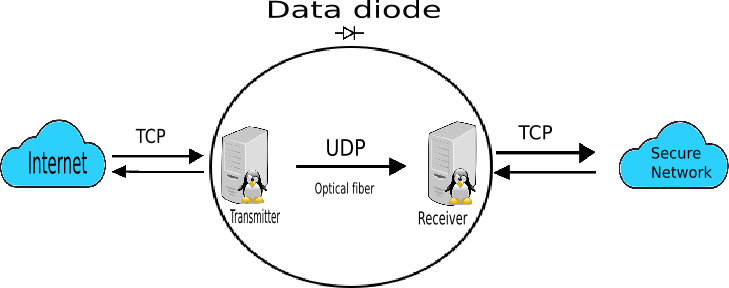
\includegraphics[scale=0.7]{img/network.png}
	\caption{High level architecture of a data diode.}
\end{figure}

\subsection{Applications}
With this data diode, we decided to keep things simple and to focus on proposing the two following services: a File Transfer service, as well as a data-diode management service. 
Other applications such as email management and web browsing will be considered for future versions of the data-diode.

\subsubsection{File Transfer}
The main application is a file transfer service that will enable files to be pushed from the outside network into the inside network, through the use of the File Transfer Protocol (FTP).

\subsubsection{Administration and Management}


\subsection{Architecture}
\subsubsection{Technical Aspects}
A data diode is composed of two servers linked by a one-way communication channel. The server, that we'll call the \textit{sender}, receives data from the external network with the TCP protocol. The second server, called the \textit{receiver}, uses the TCP protocol to send data to the secure network too. The same conclusion can then be applied to those data.\\

The one-way communication channel between the two sides of the data-diode forbids the use of a TCP based protocol (such as HTTP or FTP), as TCP requires bi-directional communication between two parties. As data between the two sides of the data-diode can only flow in one direction, we need data to be send over a protocol that doesn't require bi-directional communication. This can be done by using UDP for the communication between our two servers. The problem with UDP is that the sender cannot be sure that the receiver received the data or if the data is not corrupted. To mitigate this risk, we chose to send three times the packets of data.


\section{Users}

\section{Data Diode Administration and Management}
\end{document}